% Source: Notion page “8. 模型压缩与知识蒸馏”. Generated without rewriting its content.
\chapter{模型压缩与知识蒸馏}

\section{设计目标}

当前 Campus6 行为识别模型采用 FP32 精度进行推理，模型性能较好，但文件体积较大。为降低部署成本，本阶段采用 QAT INT8 量化 + Logits 知识蒸馏 的方案，在显著压缩模型大小的同时，尽可能保持原始模型的分类能力。

系统保留原始 FP32 Campus6 模型作为 Teacher，将经过 QAT 量化训练的模型作为 Student。Teacher 输出六维分类 logits，Student 在学习真实标签的同时学习 Teacher 的类别分布，从而补偿量化带来的精度损失。

最终流程如图所示：

\begin{figure}[htbp]
\centering
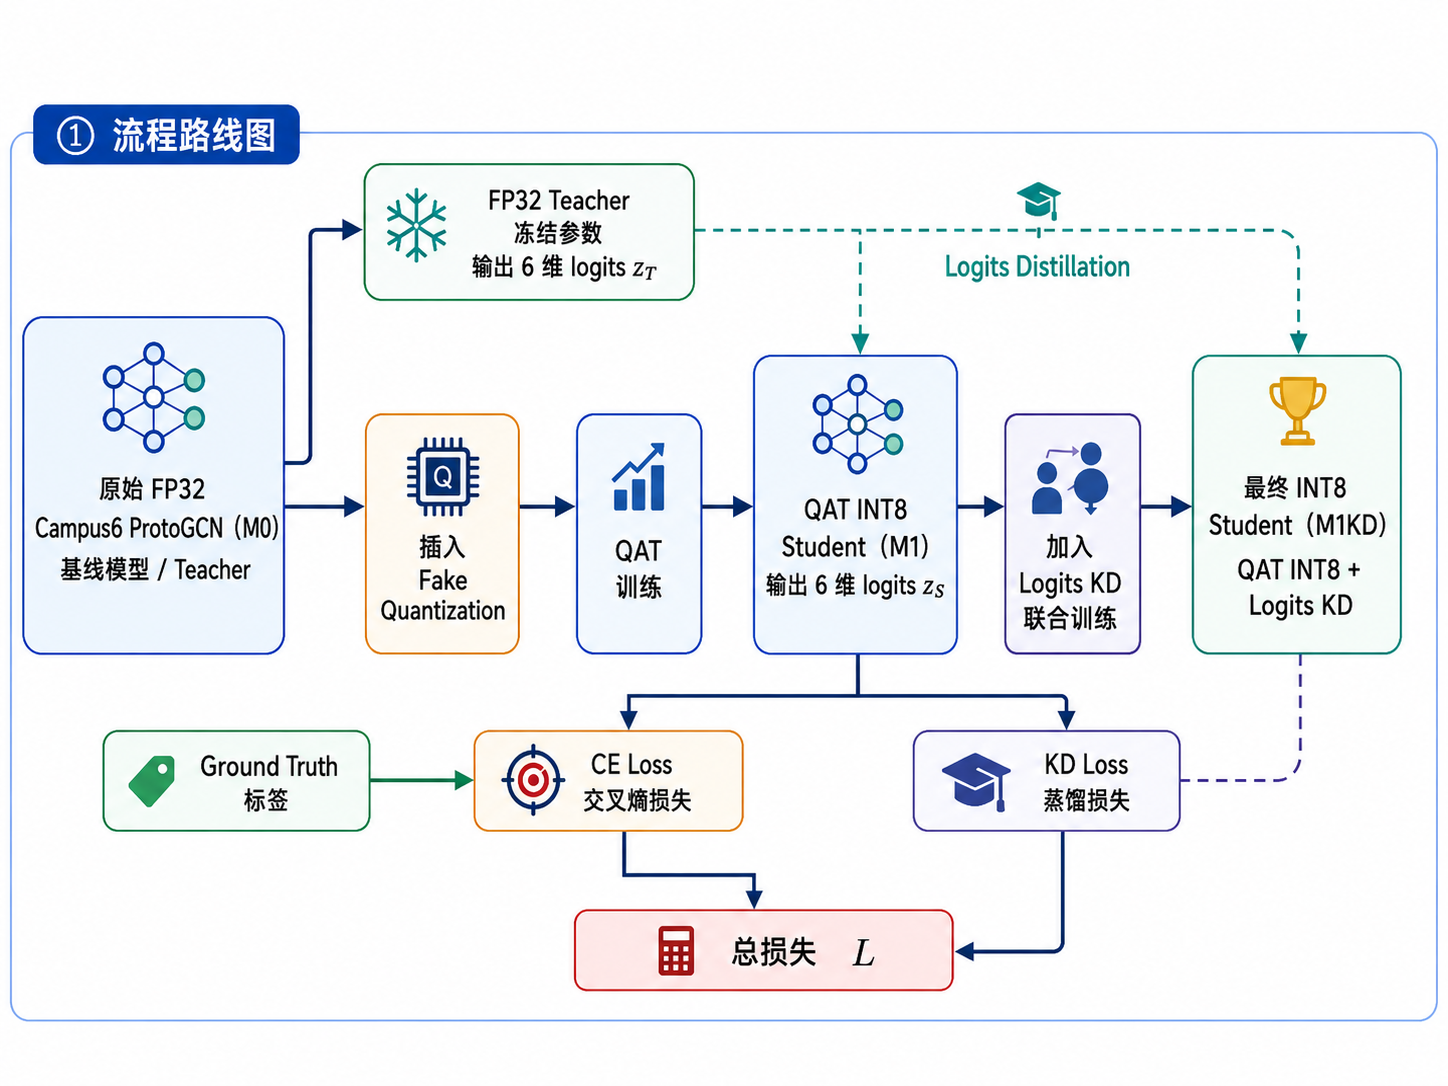
\includegraphics[width=0.96\linewidth,keepaspectratio]{figures/notion_image_05.png}
\end{figure}

\section{模型压缩方案选择}

本项目同时测试了量化与剪枝及其组合方案，结果如下：

\begin{center}
\small
\begin{longtable}{|>{\raggedright\arraybackslash}p{0.22\linewidth}|>{\raggedright\arraybackslash}p{0.22\linewidth}|>{\raggedright\arraybackslash}p{0.22\linewidth}|>{\raggedright\arraybackslash}p{0.22\linewidth}|}
\hline
模型 & Test Accuracy & ALL Accuracy & 模型部署大小 \\
\hline
M0 FP32 & 88.68\% & 96.65\% & 16.59MB \\
\hline
M1 QAT INT8 & 83.02\% & 95.81\% & 4.35 MB \\
\hline
M1I4KD：INT4 & 58.49\% & 57.82\% & 2.80 MB \\
\hline
M1I4KD：INT4 + Logits KD & 54.72\% & 56.42\% & 2.80 MB \\
\hline
M1KD QAT INT8 + Logits KD & 86.79\% & 96.37\% & 4.35 MB \\
\hline
M2 剪枝 + INT8 & 56.60\% & 78.77\% & 3.41 MB \\
\hline
M3 剪枝 + INT8 + Logits KD & 60.38\% & 72.07\% & 3.41 MB \\
\hline
\end{longtable}
\end{center}

剪枝虽然可以将模型进一步压缩至 3.41 MB，但准确率下降较大，即使加入知识蒸馏也无法恢复到可接受水平。因此最终不采用剪枝，而选择 QAT INT8 + Logits KD。该方案能够将模型从 16.30 MB 压缩至 5.31 MB，同时保持较高的识别准确率。

\section{INT8 量化设计}

原始模型采用 FP32 参数，而 INT8 使用 8 bit 表示权重和激活，因此可以显著减少模型存储空间。

本系统采用 QAT（Quantization Aware Training，量化感知训练）。训练过程中通过 Fake Quantization 模拟 INT8 的舍入和截断误差，使模型提前适应量化后的数值变化。

量化过程表示为：

\[
x_q=
\operatorname{clamp}
\left(
\operatorname{round}\left(\frac{x}{s}\right)+z
\right)
\]

其中 ss 为量化尺度，zz 为零点。

整体流程为：

\[
\begin{gathered}
\text{FP32 模型}\\[-0.2em]
\downarrow\\[-0.2em]
\text{Fake Quantization}\\[-0.2em]
\downarrow\\[-0.2em]
\text{QAT 训练}\\[-0.2em]
\downarrow\\[-0.2em]
\text{INT8 Conversion}\\[-0.2em]
\downarrow\\[-0.2em]
\text{INT8 模型}
\end{gathered}
\]

实验中，模型文件大小由 40.53 MB 降低至 5.31 MB，说明量化能够显著降低部署模型的存储占用。

\section{Logits 知识蒸馏设计}

INT8 量化会引入数值误差，因此量化后的模型可能出现一定程度的精度下降。为恢复这部分能力，本系统使用原始 FP32 模型作为 Teacher，QAT INT8 模型作为 Student。

对于同一个输入样本 xx：

\[
z_T=f_T(x)
\]

\[
z_S=f_S(x)
\]

其中：

\begin{itemize}
\item \(z_T\) 为 FP32 Teacher 输出的六维原始 logits；
\item \(z_S\) 为量化 Student 输出的六维 logits。
\end{itemize}

Teacher 在蒸馏过程中保持冻结，仅负责提供分类知识。Student 同时学习真实标签和 Teacher logits。

相比单独使用 One-hot 标签，Teacher logits 还包含不同类别之间的相对关系，因此可以帮助量化后的 Student 更好地保持原始模型的分类边界。


\section{蒸馏损失设计}

首先使用 Temperature TT 对 Teacher 和 Student 的 logits 进行平滑：

\[
p_T=softmax\left(\frac{z_T}{T}\right)
\]

\[
p_S=softmax\left(\frac{z_S}{T}\right)
\]

随后通过 KL 散度计算知识蒸馏损失：

\[
L_{KD}=T^2D_{KL}(p_T\|p_S)
\]

同时保留真实标签对应的交叉熵损失：

\[
L_{CE}=CrossEntropy(z_S,y)
\]

最终损失函数为：

\[
\lambda L_{KD}
\]

其中 \(L_{CE}\) 保证 Student 学习真实标签，\(L_{KD}\) 约束 Student 的输出分布接近原始 FP32 Teacher。

实验初始设置为：

\[
T=4,\qquad \lambda=1.0
\]

\section{QAT 与知识蒸馏联合训练}

训练阶段同时加载 FP32 Teacher 和 Fake-INT8 Student：

\[
\begin{gathered}
\text{骨架输入}\\[-0.2em]
\downarrow\\[-0.2em]
\text{FP32 Teacher}\\[-0.2em]
\downarrow\\[-0.2em]
\text{Teacher Logits}
\end{gathered}
\]

同时：

\[
\begin{gathered}
\text{骨架输入}\\[-0.2em]
\downarrow\\[-0.2em]
\text{Fake-INT8 Student}\\[-0.2em]
\downarrow\\[-0.2em]
\text{Student Logits}
\end{gathered}
\]

然后计算：

\[
\begin{gathered}
\text{Student + Ground Truth}\\[-0.2em]
\downarrow\\[-0.2em]
\text{CE Loss}
\end{gathered}
\]

\[
\begin{gathered}
\text{Teacher Logits + Student Logits}\\[-0.2em]
\downarrow\\[-0.2em]
\text{KD Loss}
\end{gathered}
\]

最终：

\[
\begin{gathered}
\text{CE Loss + KD Loss}\\[-0.2em]
\downarrow\\[-0.2em]
\text{更新 Student}
\end{gathered}
\]

Teacher 全程冻结，不参与参数更新。Student 在适应 INT8 量化误差的同时学习原始 FP32 模型的分类能力。

训练完成后，将 Student 正式转换为 INT8 模型。Teacher 仅在训练阶段使用，因此不会增加最终部署模型的大小和推理开销。

最终，普通 QAT INT8 模型的 Test Accuracy 为 83.02\%，加入 Logits 蒸馏后提高至 86.79\%，模型大小仍保持 5.31 MB。因此最终采用 QAT INT8 + Logits Knowledge Distillation 作为 Campus6 模型的轻量化方案。

注：由于int8模型置信度过高，所以我们采用温度=5来对它输出的logits进行软化

